%%%%%%%%%%%%%%%%%%%%%%%%%%%%%%%%%%%%%%%%%%%%%%%%%%%%%%%%%%%%%%%%%%%%%%%%%%%%% 
%
% This is a LaTeX file for an A0 poster.
%
% 
%%%%%%%%%%%%%%%%%%%%%%%%%%%%%%%%%%%%%%%%%%%%%%%%%%%%%%%%%%%%%%%%%%%%%%%%%%%%%
%%%%%%%%%%%%%%%%%%%%%%%%%%%%%%%%%%%%%%%%%%%%%%%%%%%%%%%%%%%%%%%%%%%%%%%%%%%%%

\documentclass[a0,portrait]{a0poster}
% To modify the size of the page:
%\usepackage{fancytikzposter} 
%\usepackage{verbatim}
\usepackage[dvips,a1paper,portrait,centering,top=1cm,bottom=-1cm,left=1cm,right=1cm]{geometry}
\usepackage{multicol}
\usepackage[latin1]{inputenc}
\usepackage{color}
\usepackage{times}
\usepackage{a0poster}
\usepackage{multirow}
\usepackage{booktabs}
%\usepackage{fixltx2e}
\usepackage{subfig}
\usepackage{graphicx} %cambiar el tamanio de la tabla
\usepackage{tabulary} %cambiar el ancho de la tabla
\usepackage{float}
%\usepackage{caption}
%\usepackage[absolute]{textpos}
\usepackage{enumitem,xcolor}
\usepackage{capt-of}

\usepackage{pdfcolparcolumns}

\usepackage{fancybox}
\usepackage{amsmath, amsthm, amsfonts}
\usepackage{graphics}           % Include figure files.

\renewcommand{\refname}{\textcolor{blue}{References}}


\usepackage{tcolorbox}% http://ctan.org/pkg/tcolorbox

\definecolor{mycolor}{rgb}{0.122, 0.435, 0.698}
\newtcbox{\mybox}{nobeforeafter,colframe=mycolor,colback=mycolor!10!white,boxrule=1pt,arc=4pt,
	boxsep=0pt,left=6pt,right=10pt,top=6pt,bottom=6pt,tcbox raise base}
% -------
\definecolor{azulillo}{rgb}{0.8,0.85,1}
\definecolor{marronrp3}{rgb}{.9,.9,.7}
\definecolor{salmon}{rgb}{1,.9,.8}
\definecolor{rojo}{rgb}{.6,.1,0}
\definecolor{ballblue}{rgb}{0.13, 0.67, 1.5}

\setlength{\parindent}{0pt}% Just for this example

\pagestyle{empty}

\def\to{\rightarrow}

% Hyphenation
\hyphenation{}


% ===========================================================================

\title{}
\author{}
\date{}

\begin{document}
%\maketitle

\begin{center}
	\begin{minipage}{.15\linewidth}
		
\includegraphics[width=.95\linewidth]{../../../../logos/LogoUNGS.JPG}
	\end{minipage}
	%&
	\hspace{.01\linewidth}
	\begin{minipage}{.65\linewidth}
		\begin{center}
			\textcolor{blue}{\huge \textbf{Gamma and Lognormal kernels with stochastic distance for texture parameter estimation under the intensity multilook $\mathcal G_I^0$ law}}\\
			\vspace{0.5cm}
			\textcolor{blue}{\large{ Julia Cassetti{\small $^1$}, Alejandro C. Frery{\small $^2$}}\\
				\textcolor{blue}{\small{$^1$Instituto del Desarrollo Humano -  Universidad Nacional de General Sarmiento}}\\
				\textcolor{blue}{\small{$^2$LaCCAN -- Laborat\'orio de Computa\c c\~ao Cient\'ifica e An\'alise Num\'erica -Universidade Federal de Alagoas}}}\\
		\end{center}
	\end{minipage}
	%&
	\hspace{.01\linewidth}
	\begin{minipage}{0.15\linewidth}
		\begin{center}
			
\includegraphics[scale=0.3]{../../../../logos/LogoUFAL.png}
		\end{center}
	\end{minipage}
\end{center}

\vspace{0.5cm}
% ---------------------------------------------------------------------------

\setlength{\columnsep}{0.05cm}
\setlength{\columnseprule}{0.05cm}
%\begin{multicols}{3}
\begin{parcolumns}[colwidths={1=.3\textwidth,2=.39\textwidth},rulebetweencolor=blue
	,rulebetween=true]{3}
\noindent
\colchunk{
%
 \begin{minipage}[t]{0.95\linewidth}
  \colorbox{salmon}{
	\begin{minipage}[t]{1\linewidth}
		   \centerline{\Large \textcolor{blue}{\textbf{Abstract}}}
		\vspace{.2cm}
		SAR imagery are well described by the $\mathcal G_I^0$ model because they possess the ability to characterize areas with different degrees of texture. 
	In the monopolarized case, this distribution depends on three parameters: the texture, the scale and the number of looks. The first one is related to the texture of the image, so its estimation deserves special attention.
	%The latter can be considered known because it can be set up during the image 		generation process, or estimated for the whole image. The first one is related to the texture of the image, so its estimation deserves special attention.
	This paper proposes and compares methods for the estimation of the texture for the multilook case. 
	This parameter is estimated by minimizing a stochastic distance between $\mathcal G_I^0$ density and an estimate of the underlying density function using Gamma and Lognormal kernels. These estimators are assessed with simulation studies. 
	The new estimators outperform the maximum likelihood estimator regarding bias and mean squared error in most cases.
	  \end{minipage}
}



%%%%%%%%%%%%%%%%%%%%%%%%%%%%%%%%%%%%%%%%%%%%%%%%%%%%%%%%%%%%%%%%%%%%
%\begin{minipage}[t]{.85\linewidth}    
\section*{\textcolor{blue}{The $\mathcal{G_I}^0$ Model}}

The return $Z$ in monopolarized SAR images can be modeled as $Z=X Y$  where $L$ is the number of looks, $X \sim \Gamma^{-1}(\alpha ,\gamma)$ corresponds to the backscatter and $Y \sim \Gamma(L,L)$ corresponds to the speckle noise. It leads to the $\mathcal{G}_I^{0}$ distribution whose density function is given by

{\small
\begin{equation*}
f_{\mathcal{G}_I^{0}}( z) =\frac{L^{L}\Gamma ( L-\alpha
	) }{\gamma ^{\alpha }\Gamma ( -\alpha ) \Gamma (
	L) }\cdot  
\frac{z^{L-1}}{( \gamma +zL) ^{L-\alpha }},%
\label{ec_dens_gI0}
\end{equation*}
}

where $-\alpha,\gamma ,z>0$ and $L\geq 1$. In this work we consider $E(Z)=1$ which links the texture and the brightness parameter by $\gamma^* =-\alpha-1$.
%The $r$-order moments are
%\begin{equation}
%\text{E}(Z^r) =\Big(\frac{\gamma}{L}\Big)^r\frac{\Gamma ( -\alpha-r )}{ \Gamma (-\alpha) }
%\frac{\Gamma (L+r )}{\Gamma (L)},
%\label{moments_gI0}
%\end{equation}
%provided $\alpha<-r$, and infinite otherwise.

\vspace{0.54cm}
%The $\alpha$ parameter is related to the texture of the target: $\alpha \in (0,-3)$ suggest extreme texture,  $\alpha \in (-6,-3]$ indicates forest zones and $\alpha\in(-\infty,-6]$ indicates homogeneous one.
%The $\gamma$ parameter is proportional to the brightness.
%With the purpose of reducing our analysis to a single parameter, we consider $E(Z)=1$ which links the texture and the brightness parameter by $\gamma^* =-\alpha-1$.



%\section*{\colorbox{blue}{\textcolor{white}{Maximum Likelihood Estimator }}}
\section*{\textcolor{blue}{Maximum Likelihood Estimator }}
%Let $Z_1,\dots, Z_n$ be an independent random sample of size $n$ from the $\mathcal G_I^0(\alpha,\gamma^*,L)$ distribution.
The maximum likelihood estimator of $\alpha$ for $L$ known, denoted $\widehat\alpha_{\text{\tiny{ML}}}$, is any value in $(-\infty,-1)$ that maximizes
{\small
	\begin{align*}
		\log \Gamma(L-\widehat\alpha_{\text{ML}})-
		\widehat\alpha_{\text{ML}}\log(-1-\widehat\alpha_{\text{ML}})
		-\log\Gamma(-\widehat\alpha_{\text{ML}}) \nonumber \\
		\mbox{}+\frac{\widehat\alpha_{\text{ML}}-L}{n} \sum_{i=1}^n\log(-1-\widehat\alpha_{\text{ML}}+L Z_i).
		\label{ML}
	\end{align*}
}
\section*{\textcolor{blue}{Stochastic distance estimator}}

\begin{center}
	\mybox{\begin{minipage}{.86\linewidth}

		$$	\widehat{\alpha}_\text{{\tiny{T}}}= \arg\min_{\alpha} d_{\text{{\tiny{T}}}}\big(f_{\tiny\mathcal{G}_I^{0}}(\alpha,\gamma^*, L ), \widehat f_\text{\tiny{K(z)}}\big)$$

		\end{minipage}
	}
\end{center}

%Cassetti et al~\cite{APSAR2013ParameterEstimationStochasticDistances} chose the triangular distance because it outperform others distances. It is defined as:
\vspace{0.5cm}
where 
\vspace{0.5cm}
\begin{center}
 \mybox{\begin{minipage}{.86\linewidth}
		$\widehat f_\text{\tiny{K(z)}}$ is a nonparametric estimation of the underlying density function using Gamma and Lognormal kernels.
	\end{minipage}
}
\end{center}
\vspace{0.5cm}
and the triangular distance is defined as
\begin{equation*}
d_{\text{\tiny{T}}}(f_\text{\tiny{V}},f_\text{\tiny{W}})=\int_{S}\frac{(f_\text{\tiny{V}}-f_\text{\tiny{W}})^2}{f_\text{\tiny{V}}+f_\text{\tiny{W}}}
\label{DT}
\end{equation*}
with $f_\text{\tiny{V}}$ and $f_\text{\tiny{W}}$ are two densities functions.

%where $d_{\tiny{\text{T}}}$ is the triangular distance defined in~\eqref{DT}, $\gamma^*$ and $L$ are known and

\end{minipage}
}
%%%%%%%%%%%%%%%%%%%%%%%%%%%%%%%%%%%%%%%%%%%%%%%%%%%%%%%%%%%%%%%%%%%%
%All the optimizations where performed using the L-BFGS-B version of the Broyden-Fletcher-Goldfarb-Shannon method.

%%%%%%%%%%%%%%%%%%%%%%%%%%%%%%%%%%%%%%%%%%%%%%%%%%%%%%%%%%%%%%%%%%%%
\colchunk{
\begin{minipage}[t]{1\linewidth}
\section*{\textcolor{blue}{Monte Carlo experiment}}
We perform  $500$ independent replications for $\alpha\in\{-1.5, -3, -5, -8\}$, $L\in\{3,8\}$, and $n\in\{9, 25,49, 81,121,500\}$, we compute the sample bias and sample mean squared error. We show the $L=3$ case, $L=8$ produces similar results.

%\section*{\textcolor{blue}{Without Contamination}}

\begin{center}
 \begin{minipage}[t]{0.90\linewidth}
  	\begin{figure}
	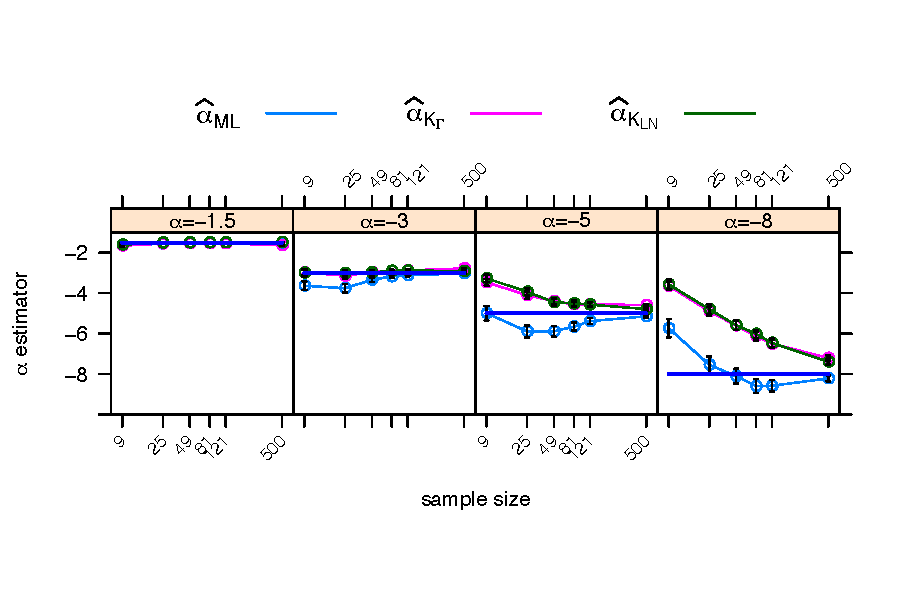
\includegraphics[width=20cm, height=12cm]{../../../../Figures/IVJIAAIS2017/SinCont/alfa500_sinmenos20_NoContMVyGAyLN_OPTIM_hasta500_MOM1_2_SinCte_Ver2_FINALbarrasdeerror_L3.pdf}\\
	\captionof*{figure}{\small{Mean value of $\widehat{\alpha}$, $L=3$.}}
	\end{figure}
\end{minipage}

	\begin{minipage}[t]{0.90\linewidth}
		\begin{figure}
  		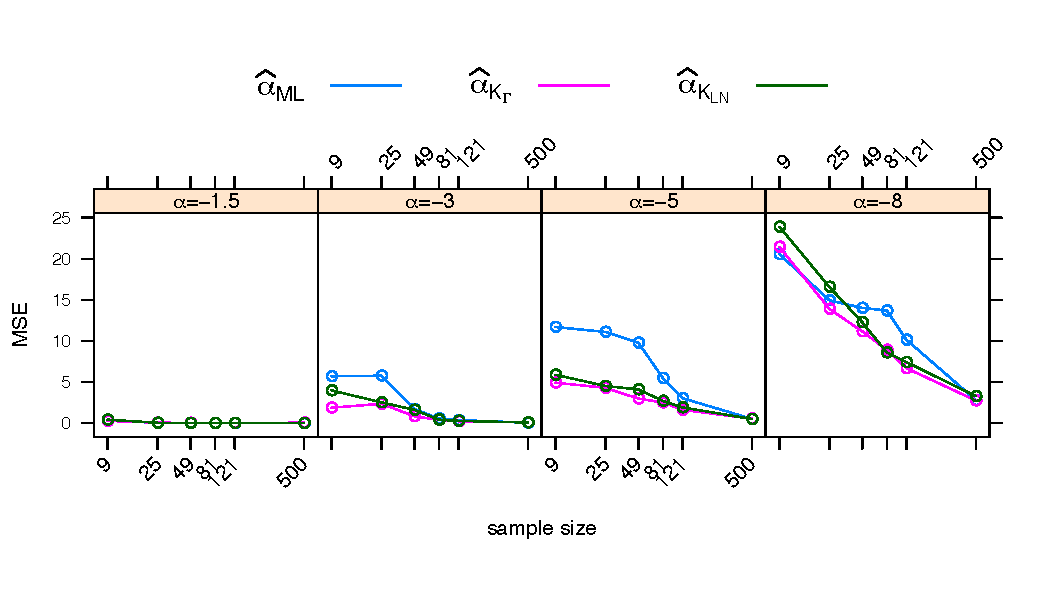
\includegraphics[width=20cm, height=12cm]{../../../../Figures/IVJIAAIS2017/SinCont/ECM_500_L3MVyGAyLN_OPTIM_hasta500_MOM1_2_SinCte_Ver2_FINAL.pdf}
  		\captionof*{figure}{\small{Mean squared error of $\widehat{\alpha}$, $L=3$.}}
 		\end{figure}
  	\end{minipage}
\end{center}

\section*{\textcolor{blue}{Robustness analysis}}
\label{robustez}
We  evaluate the robustness of the proposed estimator defining $Z=(1-B)W+BU$ where: $W \sim \mathcal{G}_I^0(\alpha,\gamma^*,L)$ is the true model, $U \sim \mathcal{G}_I^0(\alpha_1,\gamma_1^*,L)$ where $\alpha_1=-15$ and $\gamma_1^*=-\alpha_1-1$, $B \sim Ber(\epsilon)$ where $\epsilon=0.05$. 
%The cumulative distribution function of $Z$ is $(1-\epsilon) {F}_{\alpha,\gamma^*,L}(z)+\epsilon {F}_{\alpha_1,\gamma_1^*,L}(z)$.
\begin{center}
	\begin{minipage}[t]{1\linewidth}
		\begin{figure}
		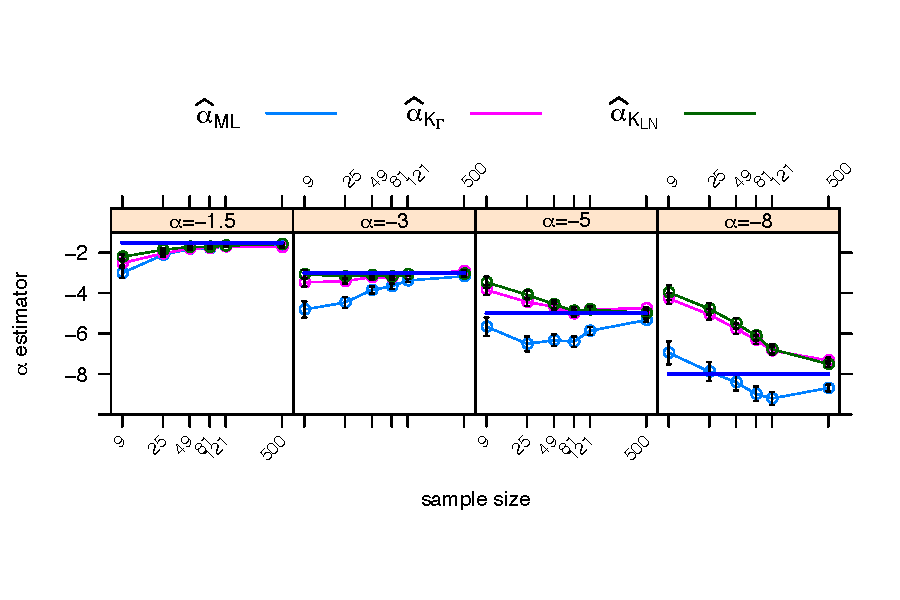
\includegraphics[width=20cm, height=12cm]{../../../../Figures/IVJIAAIS2017/Cont/alfa500_sinmenos20_CONTMVconX0yGAyLN_OPTIM_hasta500_MOM1_2_SinCte_Ver2FINALbarrasdeerror_L3.pdf}\\
		\captionof*{figure}{\small{Mean value of $\widehat{\alpha}$, $L=3$.}}
		\end{figure}
	\end{minipage}
\end{center}

	
\begin{center}
	\begin{minipage}[t]{1\linewidth}
	\begin{figure}
		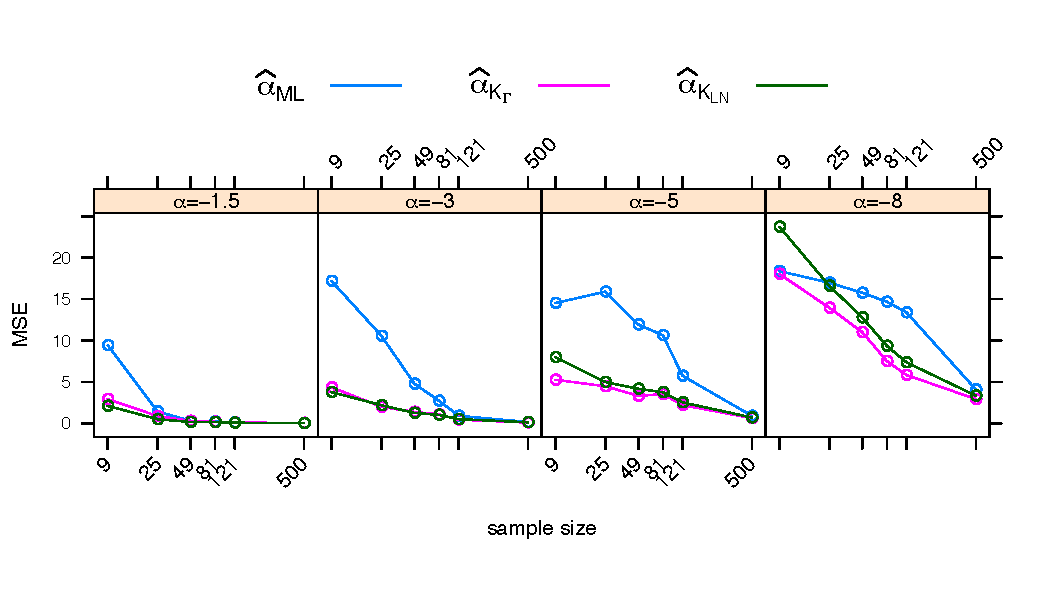
\includegraphics[width=20cm, height=12cm]{../../../../Figures/IVJIAAIS2017/Cont/ECM_500_L3MVconX0yGAyLN_OPTIM_hasta500_MOM1_2_SinCte_Ver2FINALeps05.pdf}
		\captionof*{figure}{\small{Mean squared error of $\widehat{\alpha}$, $L=3$.}}
		\end{figure}
	\end{minipage}
\end{center}
%In particular, in image processing and analysis one is seldom able to grant that the underlying hypothesis under which the techniques being employed hold, so the ability of performing well even under deviations from these assumptions is a requirement.

%	\item through EIF -- Empirical Influence Function. Fixing $n-1$ observations and allowing one to vary, but it depends on the particular sample. To avoid this, Andrews et al.~\cite{Andrews1972}, proposed using the $i^{th}$ quantile of the assumed distribution to characterize the typical observations $z_i=F^{-1}\big((i-1/3)/(n+1/3) \big)$, $1\leq i\leq n-1$.
%	This is the SEIF -- Stylized Empirical Influence Function.
%\end{itemize}
\end{minipage}
}
%%%%%%%%%%%%%%%%%%%%%%%%%%%%%%%%%%%%%%%%%%%%%%%%%%%%%%%%%%%%%%%%%%%%

%%%%%%%%%%%%%%%%%%%%%%%%%%%%%%%%%%%%%%%%%%%%%%%%%%%%%%%%%%%%%%%%%%%%
\colchunk{
\begin{minipage}[t]{\linewidth}
\section*{\textcolor{blue}{Stylized Samples}}
Empirical Influence Function shows the performance of the estimator $\widehat{\alpha}_{\text{\tiny{T}}}$ when $n-1$ observations are fixed and one ranges over the support of the distribution. It depends on the particular sample so we use the $i^{th}$ quantile of the assumed distribution to characterize the typical observations.

%Empirical Influence Function shows the performance of the estimator $\widehat{\alpha}_{\text{\tiny{T}}}$ when $n-1$ observations are fixed and one ranges over the support of the distribution. It depends on the particular sample so, to avoid this, Andrews et al.~\cite{Andrews1972} proposed using the $i^{th}$ quantile of the assumed distribution to characterize the typical observations $z_i=F^{-1}\big((i-1/3)/(n+1/3) \big)$, $1\leq i\leq n-1$.

\begin{center}
	\begin{minipage}[t]{1\linewidth}
		\begin{figure}
			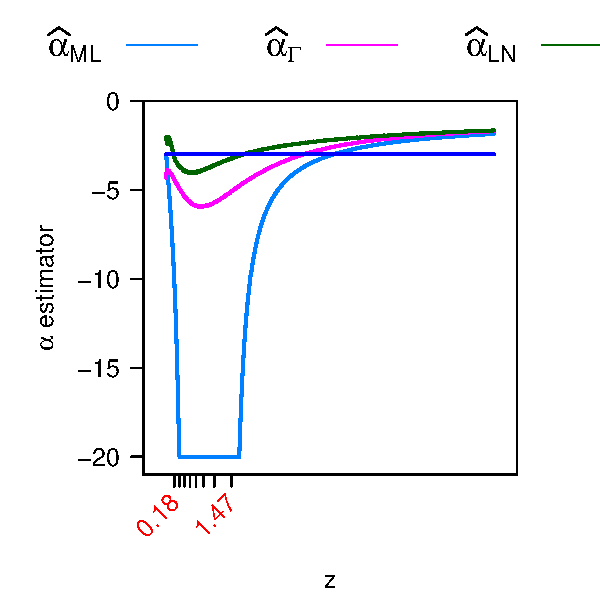
\includegraphics[scale=1.5]{../../../../Figures/IVJIAAIS2017/Cont/INFL_LNyMVyGA_alfa-3_L3n9.pdf}
			\captionof*{figure}{\small{SEIFs for $L=3$, $\alpha=-3$ and $n=9$. \label{figure:SEIFL1}}}
		\end{figure}
	\end{minipage}
\end{center}


%\begin{center}
%	\begin{minipage}[t]{0.85\linewidth}
%		\begin{figure}
%			\includegraphics[scale=1.5]{../../../../Figures/IVJIAAIS2017/CONT/INFL_LNyMVyGA_alfa-3_L3n49.pdf}
%			\captionof*{figure}{\small{SEIFs for $L=3$, $\alpha=-3$ and $n=49$.}}
%		\end{figure}
%	\end{minipage}
%\end{center}

\section*{\textcolor{blue}{Number of cases of no convergence}}
An algorithm is considered to converge if it finds an estimate $\widehat{\alpha}$ larger than $-20$.

\[
\footnotesize{
\begin{array}{c c c c}
\begin{tabulary}{5cm}{ 
	c|@{\hspace{0.9cm}} c @{\hspace{0.7cm}} c @{\hspace{0.7cm}} c @{\hspace{0.7cm}} c @{\hspace{0.5cm}} }
\hline	
$\alpha$ & $n$ & $\widehat{\alpha}_{\text{\tiny{ML}}}$ 
& $\widehat{\alpha}_{\textup{\tiny $\Gamma$}}$
& $\widehat{\alpha}_{\text{\tiny{LN}}}$\\
\hline
\multirow{6 }{*}{$-1.5\text{  }$} 
& $9$   &  $0$  & $0$  & $2$  \\ 
& $25$  &  $0$  & $0$  & $0$  \\ 
& $49$  &  $0$  & $0$  & $0$  \\ 
& $81$  &  $0$  & $0$  & $0$  \\ 
& $121$ &  $0$  & $0$  & $0$  \\ 
& $500$ &  $0$  & $0$  & $0$  \\ 
\hline
\multirow{6 }{*}{$-3$} 
& $9$   & $65$  & $25$ & $33$ \\ 
& $25$  &  $5$  &  $1$ &  $4$ \\ 
& $49$  &  $1$  &  $0$ &  $1$ \\ 
& $81$  &  $0$  &  $0$ &  $0$ \\ 
& $121$ &  $0$  &  $0$ &  $0$ \\ 
& $500$ &  $0$  &  $0$ &  $0$ \\
%\end{tabulary}
%& \hspace{0.5cm}
%\begin{tabulary}{5cm}{ 
%	c|@{\hspace{0.9cm}} c @{\hspace{0.7cm}} c @{\hspace{0.7cm}} c @{\hspace{0.7cm}} c @{\hspace{0.5cm}} }
\hline	
$\alpha$ & $n$ & $\widehat{\alpha}_{\text{\tiny{ML}}}$ 
& $\widehat{\alpha}_{\textup{\tiny $\Gamma$}}$
& $\widehat{\alpha}_{\text{\tiny{LN}}}$\\
\hline
\multirow{6 }{*}{$-5\text{  }$} 
& $9$   & $134$ & $44$ & $61$ \\ 
& $25$  & $50$  & $14$ & $24$ \\ 
& $49$  & $17$  &  $7$ &  $6$ \\ 
& $81$  &  $6$  &  $2$ &  $4$ \\ 
& $121$ &  $2$  &  $0$ &  $1$ \\ 
& $500$ &  $0$  &  $0$ &  $0$ \\ 
\hline
\multirow{6 }{*}{$-8$} 
& $9$   & $198$  & $76$ & $88$ \\ 
& $25$  & $143$  & $42$ & $54$ \\ 
& $49$  & $ 92$  & $25$ & $25$ \\ 
& $81$  & $ 60$  & $20$ & $20$ \\ 
& $121$ & $ 29$  &  $9$ & $10$ \\ 
& $500$ &  $ 0$  &  $0$ &  $1$ \\ 
%\bottomrule
\end{tabulary}
\end{array}
}
\]

 
\section*{\textcolor{blue}{Conclusions}}
\begin{itemize}
	\item[\textcolor{red}{\textbullet}] The $\widehat{\alpha}_{\text{\tiny{T}}}$ estimator perform very well for extreme textured and textured zones, as they outperform the $\widehat{\alpha}_{\text{\tiny{ML}}}$ estimator in almost all cases under study. %estimator in these cases in bias, and in all cases in mean squared error.
	%\item[\textcolor{red}{\textbullet}] The robustness of $\widehat\alpha_{\text{\tiny{T}}}$ with respect to $\widehat\alpha_{\text{\tiny{ML}}}$ was made evident by using Stylized Empirical Influence Functions.
	%\item[\textcolor{red}{\textbullet}] The robustness of $\widehat\alpha_{\text{\tiny{T}}}$ with respect to $\widehat\alpha_{\text{\tiny{ML}}}$ was made evident by using stylized samples.
	\item[\textcolor{red}{\textbullet}] The robustness of $\widehat\alpha_{\text{\tiny{T}}}$ is when stylized samples are used.
	\item[\textcolor{red}{\textbullet}] $\widehat\alpha_{\text{\tiny{T}}}$ is more computationally intensive than $\widehat\alpha_{\text{\tiny{ML}}}$.
	\item[\textcolor{red}{\textbullet}] The small bias $\widehat{\alpha}_{\text{\tiny{T}}}$ presents is remarkable even under contamination.
\end{itemize}
\end{minipage}
%%%%%%%%%%%%%%%%%%%%%%%%%%%%%%%%%%%%%%%%%%%%%%%%%%%%%%%%%%%%%%%%%%%%

%\bibliographystyle{plain}
%
%\bibliography{../../../../Bibliography/bib_julia}
}
%\end{multicols}
\end{parcolumns}

\end{document}